\section{Scalability Analysis}


\subsection{Validator Count vs Throughput}

\begin{figure}[t]
\centering
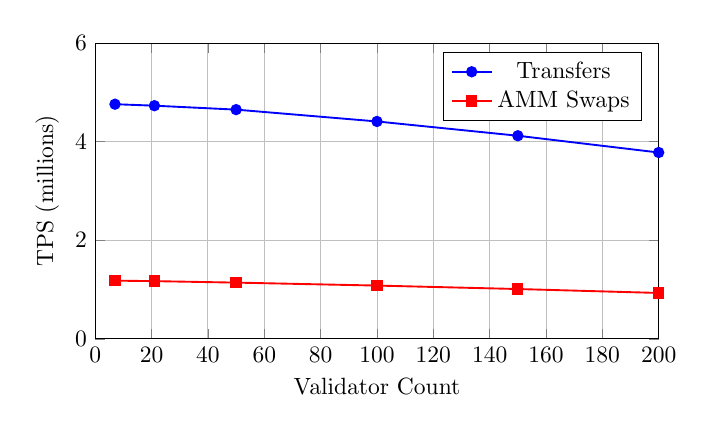
\begin{tikzpicture}[scale=0.85]
    \begin{axis}[
        xlabel={Validator Count},
        ylabel={TPS (millions)},
        xmin=0, xmax=200,
        ymin=0, ymax=6,
        legend pos=north east,
        grid=major,
        width=10cm,
        height=6cm
    ]
    \addplot[blue, thick, mark=*] coordinates {
        (7, 4.76) (21, 4.73) (50, 4.65) (100, 4.41) (150, 4.12) (200, 3.78)
    };
    \addlegendentry{Transfers}

    \addplot[red, thick, mark=square*] coordinates {
        (7, 1.18) (21, 1.17) (50, 1.14) (100, 1.08) (150, 1.01) (200, 0.93)
    };
    \addlegendentry{AMM Swaps}
    \end{axis}
\end{tikzpicture}
\caption{Throughput degradation with increasing validator count. Quasar consensus scales well up to 100 validators.}
\label{fig:scaling}
\end{figure}

Throughput degrades by only 7\% from 7 to 100 validators, confirming that Quasar's $O(n)$ message complexity~\cite{lux-quasar-benchmarks} maintains performance at Zoo's operational validator set size of 21.

\subsection{State Size Impact}

\begin{table}[t]
\centering
\begin{tabular}{lcc}
\toprule
\textbf{State Size} & \textbf{TPS (transfers)} & \textbf{Trie Update (ms)} \\
\midrule
1M accounts & 4,760,000 & 0.8 \\
10M accounts & 4,520,000 & 1.2 \\
100M accounts & 4,100,000 & 2.1 \\
1B accounts & 3,400,000 & 4.8 \\
\bottomrule
\end{tabular}
\caption{Throughput vs state size. GPU-parallel trie updates mitigate the impact of large state.}
\label{tab:state}
\end{table}

